\chapter{Sistemi operativi: struttura e servizi}
\subsubsection{Argomenti}
\begin{itemize}
    \item A che servono i sistemi operativi?
    \item Requisiti per i sistemi operativi
    \item Struttura e servizi dei sistemi operativi
    \item Chiamate di sistema ed API
    \item I programmi di sistema
\end{itemize}

\section{I sistemi operativi}
Un S.O. è una certa quantità di software che viene dato assieme all'hardware perché quest'ultimo da solo non funziona. Per esempio quando compri un telefonino apri e ti trovi Android o iOS, mentre su un laptop abbiamo Windows, macOS e Linux.\\ 
Parliamo del modello teorico della macchina di Von Neumann. Questo modello si basa su cinque componenti fondamentali:
\begin{itemize}
    \item Unità centrale di elaborazione (\textbf{CPU}), che si divide a sua volta in unità aritmetica e logica (ALU o unità di calcolo) e unità di controllo;
    \item Unità di \textbf{memoria}, intesa come memoria di lavoro o memoria principale (RAM, Random Access Memory);
    \item Unità di \textbf{input}, tramite la quale i dati vengono inseriti nel calcolatore per essere elaborati;
    \item Unità di \textbf{output}, necessaria affinché i dati elaborati possano essere restituiti all'operatore;
    \item \textbf{Bus}, un canale che collega tutti i componenti fra loro.
\end{itemize}
Un computer quando lo accendiamo inizia ad eseguire un programma. Se non c'è un programma da eseguire è solo un mucchio di ferraglia che si blocca e non fa niente. Perciò possiamo dire che un S.O. è il \textbf{primo} programma che viene eseguito all'accensione del computer e che permette di eseguire altri programmi. \`E una cosa molto diversa dalle \textit{applicazioni}, che sono quelle che "fanno le cose utili" cit prof. Infatti la prima cosa che facciamo quando per esempio compriamo un telefono è installare WhatsApp o altre app che ci servono e rendono comomda la vita. Un S.O. di per sé non è \textit{"utile"}, lo diventa in relazione al funzionamento delle app che ci interessano.\\
Un S.O. fornisce un ambiente a finestre (laptop) o icone (smartphone) che permette di eseguire le applicazioni utili: le possiamo installare, lanciare, far eseguire (anche più di una contemporaneamente), interromperne l'esecuzione\dots\\
La macchina di Von Neumann esegue un programma alla volta, ma noi di solito su un computer eseguiamo più di un'applicazione alla volta (es. WebEx per la lezione e VSCode per gli appunti). Questa cosa ci è permessa dal S.O., che ci permette ci gestire \textit{n} applicazioni contemporaneamente, anche più dei processori di cui dispone il mio computer. Es.: mettiamo di avere un computer con un processore a 32 core, io però posso eseguire anche centinaia di programmi contemporaneamente, non massimo 32.\\
Il S.O. crea un'ambiente in cui le applicazioni possono collaborare assieme. Se avessi più applicazioni che usano contemporaneamente lo stesso hardware (es. lo schermo)? Il S.O. si occupa di gestire le risorse hardware e di farle usare alle applicazioni. Il S.O. è il software \textit{intermediario} tra le applicazioni e l'hardware.\\
Un'altra cosa che fa il S.O. è organizzare i nostri file in un sistema ordinato di file e cartelle (anche memorizzandoli su dispositivi secondari di memoria e storaging). Il S.O. si occupa di gestire i file e le cartelle, di crearli, cancellarli, rinominarli, spostarli\dots 

\subsubsection{Cos'è un sistema opertativo?}
È un insieme di programmi (software) che gestiscono gli elementi fisici di un computer (hardware).\\
\vspace{5mm}
Fornisce una piattaforma di sviluppo per le applicazioni, che permette loro di condividere ed astrarre le risorse hardware.\\
Agisce da intermediario tra utenti e computer, permettendo agli utenti di controllare l'esecuzione dei programmi applicativi e l'assegnazione delle risorse hardware ad essi.\\
Protegge le risorse degli utenti (e dei loro programmi) dagli altri utenti (e dai loro programmi) e da eventuali attori esterni.\\
\vspace{5mm}
Un S.O. in primo luogo è una piattaforma di sviluppo, ossia \textbf{un insieme di funzionalità software} che i programmi applicativi possono usare.\\
Tali funzionalità permettono ai programmi di poter usare in maniera conveniente le risorse hardware, e di condividerle:
\begin{itemize}
    \item Da un lato, il S.O. \textbf{astrae} le risorse hardware, presentando agli sviluppatori dei programmi applicativi una visione delle risorse hardware più facile da usare e più potente rispetto alle risorse hardware «native».
    \item Dall'altro, il S.O. \textbf{condivide} le risorse hardware tra molti programmi contemporaneamente in esecuzione, suddividendole tra i programmi in maniera equa ed efficiente e controllando che questi le usino correttamente.
\end{itemize}

\subsubsection{Componenti di un sistema di elaborazione}
\begin{center}
    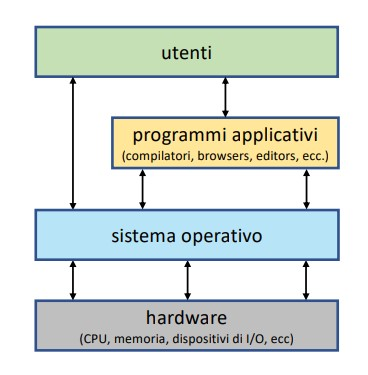
\includegraphics[width=35mm]{images/SO/SO_sistema_di_elaborazione1.jpg}
\end{center}
Utenti: persone, macchine, altri computer\dots\\
Programmi applicativi: risolvono i problemi di calcolo degli utenti.\\
S.O.: coordina e controlla l'uso delle risorse hardware.\\
Hardware: risorse di calcolo (CPU, periferiche, memorie di massa\dots).

\subsection{Requisiti per i sistemi operativi}
\subsubsection{Cosa si richiede ad un S.O.?}
Oggigiorno i computer sono ovunque: vi sono molteplici tipologie di computer utilizzati in scenari applicativi diversi (i nostri laptop, i nostri smartphones, i computer detti "embedded" che non hanno lo scopo di interagire con persone ma sono "cyber-fisici", cioè che fanno parte di servizi ad es. quelli che controllano le automobili ad es. il sistema ABS che fa in modo che la ruota non si blocchi e quindi non slitti quando noi inchiodiamo e freniamo a fondo, etc\dots).\\
In quasi tutti i tipi di computer si tende ad installare un S.O. allo scopo di gestire l'hardware e semplificare la programmazione.\\
Ma ogni scenario applicativo in cui viene usato un computer richiede che il S.O. che vi viene installato abbia caratteristiche ben determinate (es. laptop molto diverso dai sistemi embedded). Che cosa si richiede ad un S.O. per supportare un certo scenario applicativo?\\
A seconda che sia: 
\begin{description}
    \item[Server, mainframe:] massimizzare la performance, rendere equa la condivisione delle risorse tra molti utenti
    \item[Laptop, PC, tablet:] massimizzare la facilità d'uso e la produttività della singola persona che lo usa
    \item[Dispositivi mobili:] ottimizzare i consumi energetici e la connettività
    \item[Sistemi embedded:] funzionare senza, o con minimo, intervento umano e reagire in tempo reale agli stimoli esterni (interrupt)
\end{description}
\subsubsection{La maledizione della generalità}
Nella storia (ed anche oggi) alcuni sistemi operativi sono stati utilizzati per scenari applicativi diversi,\\
Ad esempio, Linux è usato oggi nei server, nei computer desktop e nei dispositivi mobili (come parte di Android).\\
La \textbf{maledizione della generalità} afferma che, se un S.O. deve supportare un insieme di scenari applicativi troppo ampio, non sarà in grado di supportare nessuno di tali scenari particolarmente
bene. Praticamente io quando cerco di dare più di un esame per sessione.\\
Questo si è visto con OS/360, il primo S.O. che doveva supportare una famiglia di computer diversi (la linea 360 dell'IBM).\\
Quella \textbf{maledizione della generalità} non avviene sempre e necessariamente, è un potenziale rischio; può essere tuttavia aggirata, ma non ho capito come.

\section{Struttura dei sistemi operativi}
Non c'è una definizione universalmente accettata di quali programmi fanno parte di un S.O..\\
In generale però un S.O. comprende almeno:
\begin{description}
    \item[Kernel:] il "programma sempre presente", che si "impadronisce" dell'hardware, lo gestisce, ed offre ai programmi i servizi per poterlo usare in maniera condivisa ed astratta.
    \item[Middleware:] servizi di alto livello che astraggono ulteriormente i servizi del kernel e semplificano la programmazione di applicazioni (API, framework per grafica e per suono\dots)
    \item[Programmi di sistema:] non sempre in esecuzione, offrono ulteriori funzionalità di supporto e di interazione utente con il sistema (gestione di jobs e processi, interfaccia utente\dots)
\end{description}
Alcuni sistemi operativi forniscono anche dei programmi applicativi (editor, word processor, fogli di calcolo…), ma non li considereremo parti del S.O. stesso.
\begin{center}
    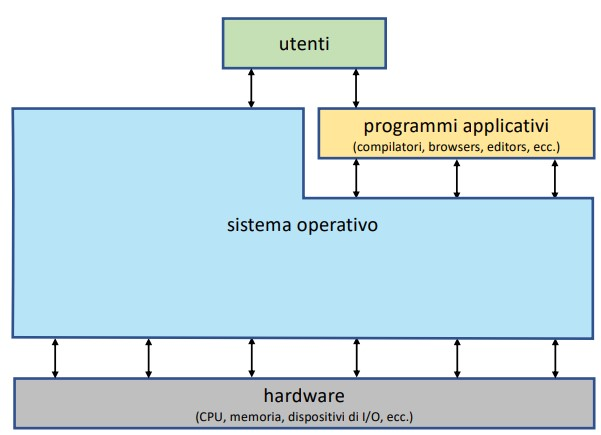
\includegraphics[width=35mm]{images/SO/SO_sistema_di_elaborazione2.jpg}
\end{center}
\begin{center}
    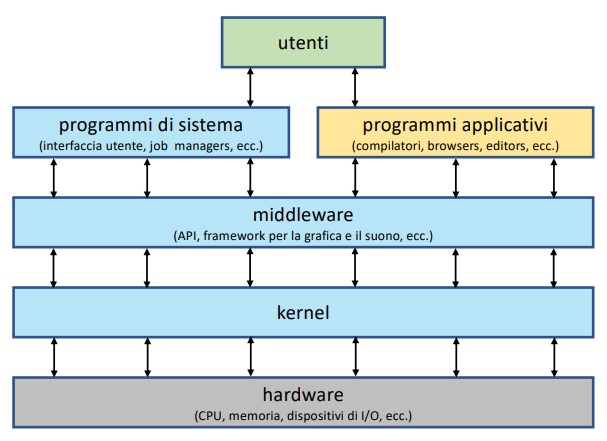
\includegraphics[width=35mm]{images/SO/SO_sistema_di_elaborazione3.jpg}
\end{center}

\section{Servizi dei sistemi operativi}
Un S.O. offre un certo numero di \textbf{servizi}:
\begin{description}
    \item[Per i programmi applicativi:] perché possano eseguire sul sistema di elaborazione usando le risorse astratte esposte dal S.O..
    \item[Per gli utenti:] per gestire l'esecuzione dei programmi e stabilire a quali risorse hardware i programmi (e gli altri utenti) hanno diritto.
    \item[] Per garantire che il sistema di elaborazione funzioni in maniera efficiente.    
\end{description}
Gli utenti però interagiscono con il S.O. attraverso i programmi di sistema\dots\\
\dots i quali utilizzano gli stessi servizi dei programmi applicativi\dots\\
Quindi, in definitiva, il S.O. ha bisogno di esporre i suoi servizi esclusivamente ai programmi (applicativi o di sistema).

\subsection{Principali servizi:}
\begin{description}
    \item[Controllo processi:] questi servizi permettono di caricare in memoria un programma, eseguirlo, identificare la sua terminazione e registrarne la condizione di terminazione (normale o erronea).
    \item[Gestione file:] questi servizi permettono di leggere, scrivere, e manipolare files e directory
    \item[Gestione dispositivi:] questi servizi permettono ai programmi di effettuare operazioni di input/output, ad esempio leggere da/scrivere su un terminale.
    \item[Comunicazione tra processi:] i programmi in esecuzione possono collaborare tra di loro scambiandosi informazioni: questi servizi permettono ai programmi in esecuzione di comunicare.
    \item[Protezione e sicurezza:] permette ai proprietari delle informazioni in un sistema multiutente o in rete di controllarne l'uso da parte di altri utenti e di difendere il sistema dagli accessi illegali.
    \item[Allocazione delle risorse:] alloca le risorse hardware (CPU, memoria, dispositivi di I/O) ai programmi in esecuzione in maniera equa ed efficiente.
    \item[Rilevamento errori:] gli errori possono avvenire nell'hardware o nel software (es. divisione per zero); quando avvengono il S.O. deve intraprendere opportune azioni (recupero, terminazione del programma o segnalazione della condizione di errore al programma).
    \item[Logging:] mantiene traccia di quali programmi usano quali risorse, allo scopo di contabilizzarle, ovvero fare sì che un programma o un utente non usi troppe risorse sottraendole ad altri programmi o utenti.
\end{description}

\section{Chiamate di sistema e API}
I programmi applicativi accedono a questi servizi che abbiamo appena elencato tramite chiamate di sistema o API.\\
Un programma applicativo che vuole accedere ai servizi offerti dal kernel non chiama direttamente dal kernel ma passa da un Middleware.\\
Il kernel offre i propri servizi ai programmi come chiamate di sistema, ossia di funzioni invocabili in un determinato linguaggio di programmazione (C, C++\dots).\\
I programmi però non utilizzano direttamente le chiamate di sistema, ma delle librerie di middleware dette Application Program Interface (API) implementate invocando le chiamate di sistema.\\
Questo perché le chiamate di sistema dipendono dal linguaggio mentre le API sono più standardizzate (es. le POSIX, tipicamente in C). Spesso le API sono fortemente legate con le librerie standard del linguaggio di implementazione (es. libc se le API sono implementate in C), al punto che anche queste diventano una parte implicita dell'API.
\begin{center}
    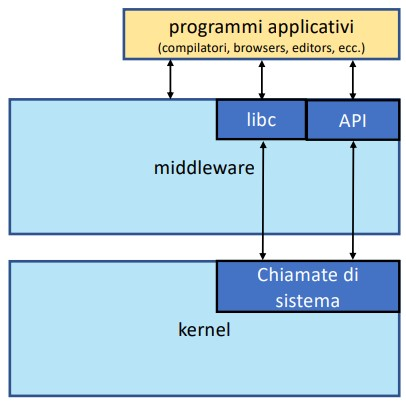
\includegraphics[width=35mm]{images/SO/SO_chiamatedisistema_API1.jpg}
\end{center}

\subsubsection{Differenza tra chiamate di sistema ed API}
Le API sono esposte dal middleware, le chiamate di sistema dal kernel.\\
Le API usano le chiamate di sistema nella loro implementazione.\\
Le API sono standardizzate (esempio: standard POSIX e Win32), le chiamate di sistema no (ogni kernel ha le sue).\\
Le API sono stabili, le chiamate di sistema possono variare al variare della versione del S.O..\\
Le API offrono funzionalità più ad alto livello e più semplici da usare, le chiamate di sistema offrono funzionalità più elementari e più complesse da usare.

\subsubsection{Esempio confronto API Win32 e POSIX}
\begin{center}
    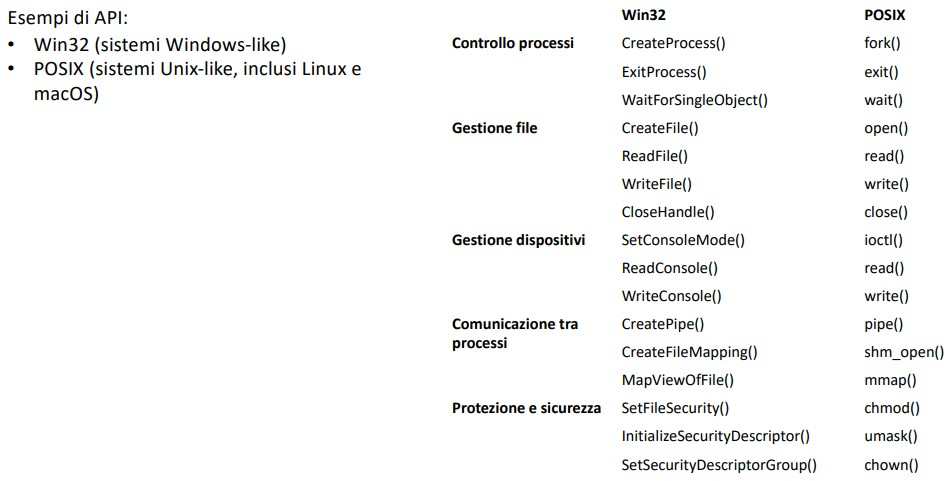
\includegraphics[width=35mm]{images/SO/SO_chiamatedisistema_API_es1.jpg}
\end{center}

\subsubsection{Esempio API POSIX}
\begin{center}
    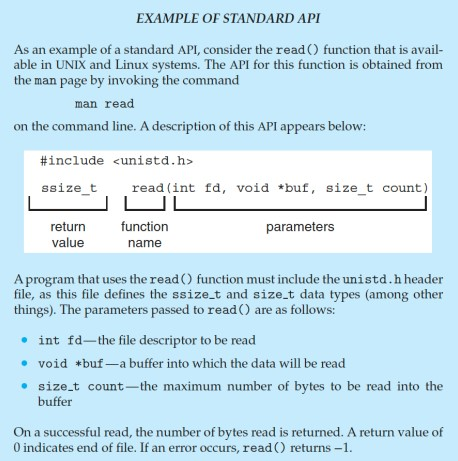
\includegraphics[width=35mm]{images/SO/SO_chiamatedisistema_API_es2.jpg}
\end{center}

\section{I programmi di sistema}
La maggior parte degli utenti utilizza i servizi del S.O. attraverso i programmi di sistema.\\
Questi permettono agli utenti di avere un ambiente più conveniente per l'esecuzione dei programmi, il loro sviluppo, e la gestione delle risorse del sistema.
\subsection{Tipologie di programmi di sistema}
\begin{description}
    \item[Interfaccia utente (UI):] permette agli utenti di interagire con il sistema stesso; può essere grafica (GUI) o a riga di comando (CLI); i sistemi mobili hanno un'interfaccia touch.
    \item[Gestione file:] creazione, modifica, e cancellazione file e directory.
    \item[Modifica dei file:] editor di testo, programmi per la manipolazione del contenuto dei file.
    \item[Visualizzazione e modifica informazioni di stato:] data, ora, memoria disponibile, processi, utenti\dots fino informazioni complesse su prestazioni, accessi al sistema e debug. Alcuni sistemi implementano un \textbf{registry}, ossia un database delle informazioni di configurazione.
    \item[Caricamento ed esecuzione dei programmi:] loader assoluti e rilocabili, linker, debugger.
    \item[Ambienti di supporto alla programmazione:] compilatori, assemblatori, debugger, interpreti per diversi linguaggi di programmazione.
    \item[Comunicazione:] forniscono i meccanismi per creare connessioni tra utenti, programmi e sistemi; permettono di inviare messaggi agli schermi di un altro utente, di navigare il web, di inviare messaggi di posta elettronica, di accedere remotamente ad un altro computer, di trasferire file\dots
    \item[Servizi in background:] lanciati all'avvio, alcuni terminano, altri continuano l'esecuzione fino allo shutdown. Forniscono servizi quali verifica dello stato dei dischi, scheduling di jobs, logging\dots
\end{description}

\subsubsection{Interfaccia utente: l'interprete dei comandi}
L'interprete dei comandi permette agli utenti di impartire in maniera testuale delle istruzioni al S.O..\\
In molti sistemi operativi è possibile configurare quale interprete dei comandi usare, nel qual caso è detto \textbf{shell}.\\
Due modi per implementare un comando:
\begin{description}
    \item[Built-in:] l'interprete esegue direttamente il comando (tipico nell'interprete di comandi di Windows)
    \item[Come programma di sistema:] l'interprete manda in esecuzione il programma (tipico delle shell Unix e Unix-like)
\end{description}
Spesso riconosce un vero e proprio linguaggio di programmazione con variabili, condizionali, cicli\dots
\begin{center}
    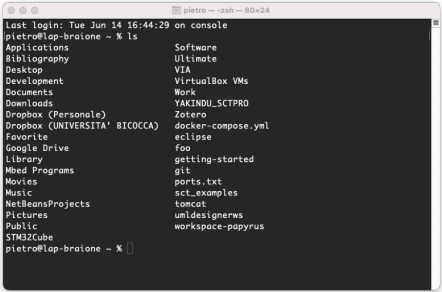
\includegraphics[width=35mm]{images/SO/SO_InterfacciaUtente_InterpreteComandi.jpg}
\end{center}

\subsubsection{Interfaccia utente: le interfacce grafiche}
L'interfaccia grafica (GUI) è di solito basata sulla metafora della scrivania, delle icone e delle cartelle (corrispondenti alle directory).\\
Nate dalla ricerca presso lo Xerox PARC lab negli anni 70, popolarizzate dal computer Apple Macintosh negli anni 80.\\
Su Linux le più popolari sono Gnome e KDE.
\begin{center}
    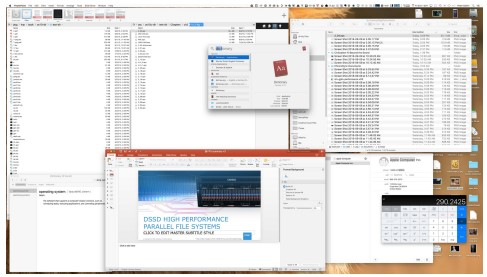
\includegraphics[width=35mm]{images/SO/SO_InterfacciaUtente_InterfacceGrafiche.jpg}
\end{center}

\subsubsection{Interfaccia utente: le interfacce touch-screen}
I dispositivi mobili richiedono interfacce di nuovo tipo.\\
Nessun dispositivo di puntamento (mouse)\\
Uso dei gesti (gestures)\\
Tastiere virtuali\\
Comandi vocali
\begin{center}
    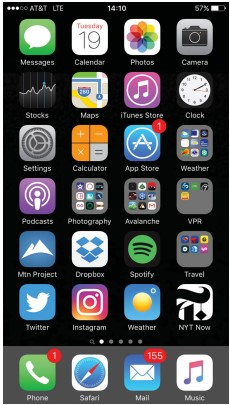
\includegraphics[width=35mm]{images/SO/SO_InterfacciaUtente_InterfacceTouchScreen.jpg}
\end{center}

\subsubsection{L'implementazione dei programmi di sistema}
I programmi di sistema sono implementati utilizzando le API, esattamente come i programmi applicativi.\\
Consideriamo ad esempio il comando cp delle shell dei sistemi operativi Unix-like:
\begin{itemize}
    \item cp in.txt out.txt
    \item Copia il contenuto del file in.txt in un file out.txt
    \item Se il file out.txt esiste, il contenuto precedente viene cancellato, altrimenti out.txt viene creato    
\end{itemize}
\`E implementato come programma di sistema.\\
Una possibile struttura del codice è riportata sulla destra (le invocazione delle API sono riportate in grassetto).
\begin{center}
    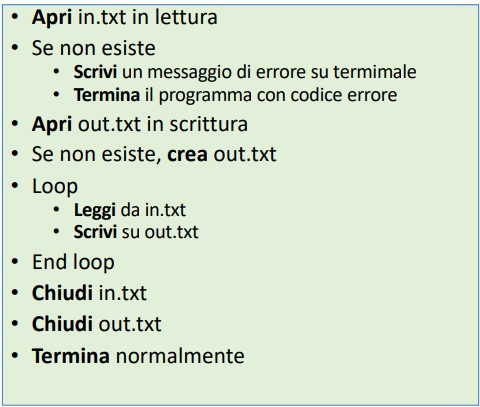
\includegraphics[width=35mm]{images/SO/SO_InterfacciaUtente_ProgrammiDiSistema.jpg}
\end{center}